\documentclass[tikz,border=4pt]{standalone}
\usepackage{libertine}
\usetikzlibrary{arrows.meta,calc,positioning,fit,backgrounds,shapes.geometric}
\definecolor{paperink}{HTML}{263441}
\definecolor{papermuted}{HTML}{647481}
\definecolor{paperline}{HTML}{CCD5DB}
\definecolor{paperblue}{HTML}{2D5F91}
\definecolor{paperbluefill}{HTML}{EFF5FA}
\definecolor{paperorange}{HTML}{B66731}
\definecolor{paperorangefill}{HTML}{FCF4EB}
\definecolor{papergreen}{HTML}{3F7558}
\definecolor{papergreenfill}{HTML}{EFF6F1}
\tikzset{
  papertext/.style={font=\footnotesize, text=paperink},
  papermini/.style={font=\scriptsize, text=papermuted},
  paneltitle/.style={font=\footnotesize\bfseries, text=paperink},
  bluebox/.style={draw=paperblue, fill=paperbluefill, rounded corners=1pt,
    line width=.6pt, font=\footnotesize, text=paperink, align=center,
    inner xsep=6pt, inner ysep=5pt},
  orangebox/.style={draw=paperorange, fill=paperorangefill, rounded corners=1pt,
    line width=.6pt, font=\footnotesize, text=paperink, align=center,
    inner xsep=6pt, inner ysep=5pt},
  greenbox/.style={draw=papergreen, fill=papergreenfill, rounded corners=1pt,
    line width=.6pt, font=\footnotesize, text=paperink, align=center,
    inner xsep=6pt, inner ysep=5pt},
  graybox/.style={draw=paperline, fill=white, rounded corners=1pt,
    line width=.6pt, font=\footnotesize, text=paperink, align=center,
    inner xsep=6pt, inner ysep=5pt},
  orangeflow/.style={-{Stealth[length=2mm]}, draw=paperorange, line width=1pt},
  blueflow/.style={-{Stealth[length=2mm]}, draw=paperblue, line width=1.15pt},
  greenflow/.style={-{Stealth[length=2mm]}, draw=papergreen, line width=1pt},
  grayflow/.style={-{Stealth[length=1.8mm]}, draw=papermuted, line width=.65pt}
}

\begin{document}
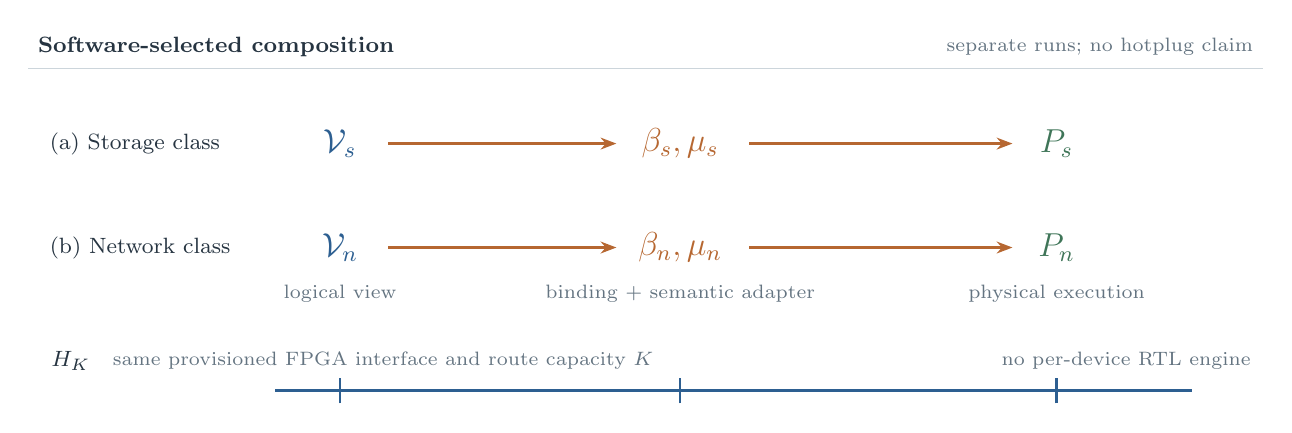
\begin{tikzpicture}[x=1cm,y=1cm]
  % Two instantiations of one capacity-bounded mechanism, not two FPGA builds.
  \node[paneltitle, anchor=west] at (.18,4.83) {Software-selected composition};
  \node[papermini, anchor=east] at (15.86,4.83) {separate runs; no hotplug claim};
  \draw[paperline] (.18,4.55) -- (15.86,4.55);

  \node[papertext, anchor=west] at (.33,3.60) {(a) Storage class};
  \node[font=\large, text=paperblue] at (4.14,3.60) {$\mathcal{V}_{s}$};
  \node[font=\large, text=paperorange] at (8.46,3.60) {$\beta_s,\mu_s$};
  \node[font=\large, text=papergreen] at (13.24,3.60) {$P_s$};
  \draw[orangeflow] (4.75,3.60) -- (7.65,3.60);
  \draw[orangeflow] (9.34,3.60) -- (12.68,3.60);

  \node[papertext, anchor=west] at (.33,2.28) {(b) Network class};
  \node[font=\large, text=paperblue] at (4.14,2.28) {$\mathcal{V}_{n}$};
  \node[font=\large, text=paperorange] at (8.46,2.28) {$\beta_n,\mu_n$};
  \node[font=\large, text=papergreen] at (13.24,2.28) {$P_n$};
  \draw[orangeflow] (4.75,2.28) -- (7.65,2.28);
  \draw[orangeflow] (9.34,2.28) -- (12.68,2.28);
  \node[papermini] at (4.14,1.69) {logical view};
  \node[papermini] at (8.46,1.69) {binding + semantic adapter};
  \node[papermini] at (13.24,1.69) {physical execution};

  \draw[paperblue, line width=1pt] (3.32,.46) -- (14.96,.46);
  \foreach \x in {4.14,8.46,13.24} {
    \draw[paperblue, line width=.85pt] (\x,.30) -- (\x,.62);
  }
  \node[papertext, anchor=west] at (.35,.84) {$H_K$};
  \node[papermini, anchor=west] at (1.13,.84)
    {same provisioned FPGA interface and route capacity $K$};
  \node[papermini, anchor=east] at (15.83,.84)
    {no per-device RTL engine};
\end{tikzpicture}
\end{document}
